\documentclass{article}
\usepackage[left=3cm,right=3cm,top=2cm,bottom=2cm]{geometry} % page settings
\usepackage{amsmath,amsthm,mathtools}
\usepackage{amsfonts,amssymb,latexsym}
\usepackage{upgreek}

\usepackage[spanish]{babel}
\usepackage[doument]{ragged2e}

\usepackage{float}

\setcounter{tocdepth}{2}

\selectlanguage{spanish}
\usepackage[utf8]{inputenc}
\setlength{\parindent}{0mm}

\usepackage[bookmarks=true,
            bookmarksnumbered=false, % true means bookmarks in 
            bookmarksopen=false,     % true means only level 1
                                     % are displayed.
            colorlinks=true,
            linkcolor=blue,
            urlcolor=cyan,
            citecolor=green]{hyperref}

\begin{document}

\title{Instalación y configuración de Zabbix}
\author{David Cabezas Berrido}
\date{}
\maketitle
\tableofcontents

\newpage

\section{Introducción}

Procederemos a instalar y configurar Zabbix 3.4 en la máquina virtual
de Ubuntu Server para monitorizar los servicios de ssh y php
tanto en la propia máquina como en la de CentOs.

\section{Instalación y configuración en UbuntuServer}

He seguido las instrucciones de la documentación
\url{https://www.zabbix.com/documentation/3.4/manual/installation/install_from_packages/debian_ubuntu}
para instalar y configurar el servidor, la base de datos, el frontend
y el agente.

\subsubsection*{Añadir repositorio de Zabbix}

\begin{figure}[H]
  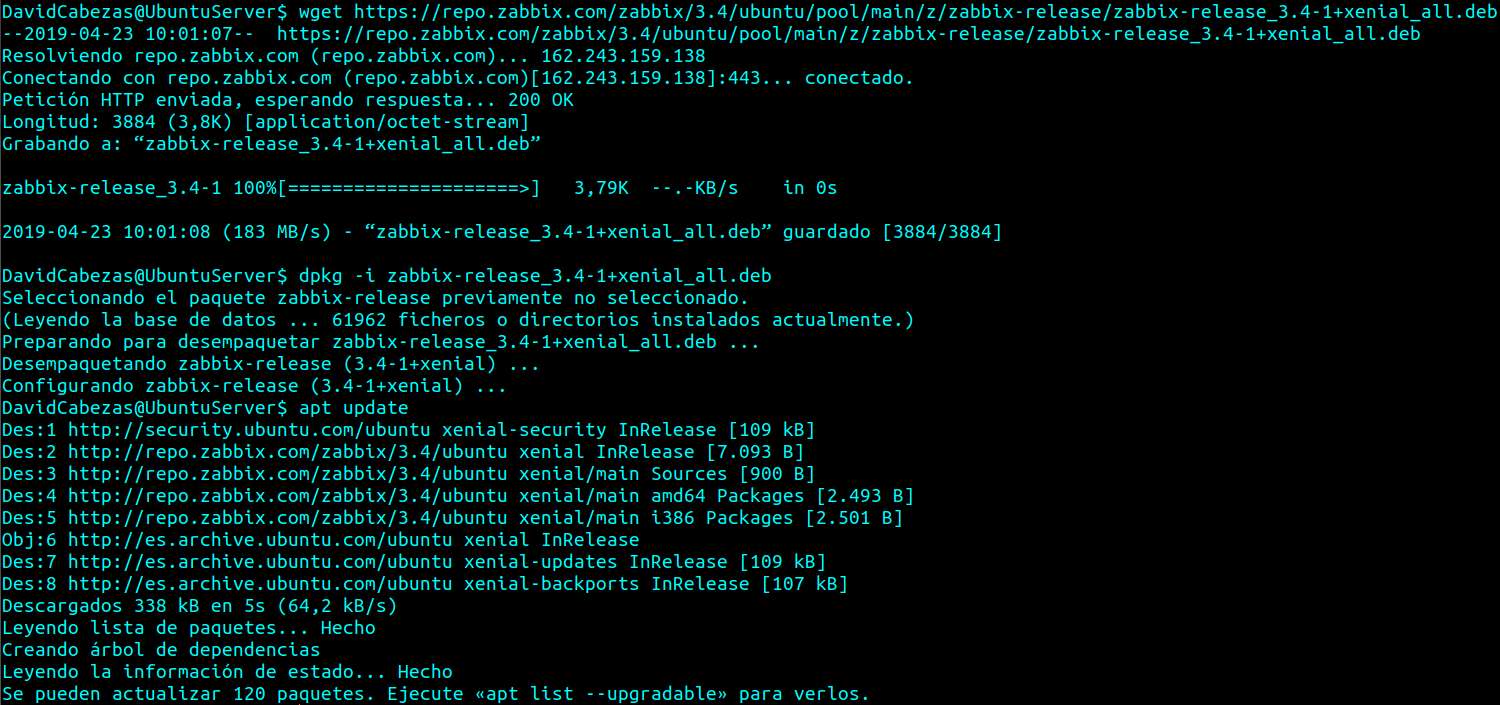
\includegraphics[width=160mm]{screenshots/paquetes}
\end{figure}

\subsubsection*{Instalar server con soporte MySQL}

\begin{figure}[H]
  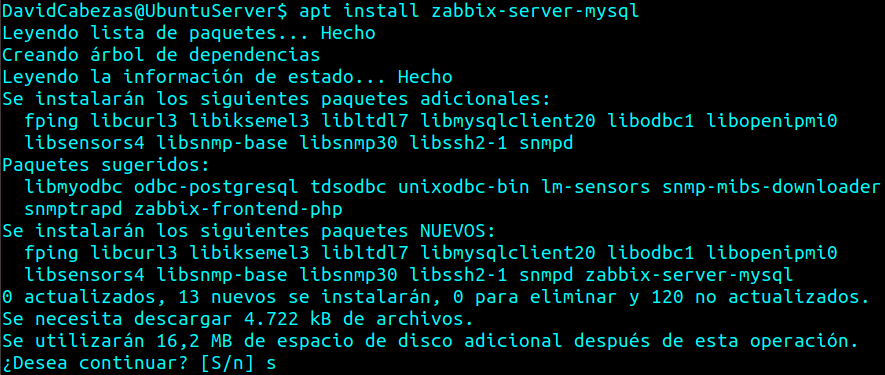
\includegraphics[width=160mm]{screenshots/server-MySQL_installation}
\end{figure}


\subsubsection*{Instalar frontend}

\begin{figure}[H]
  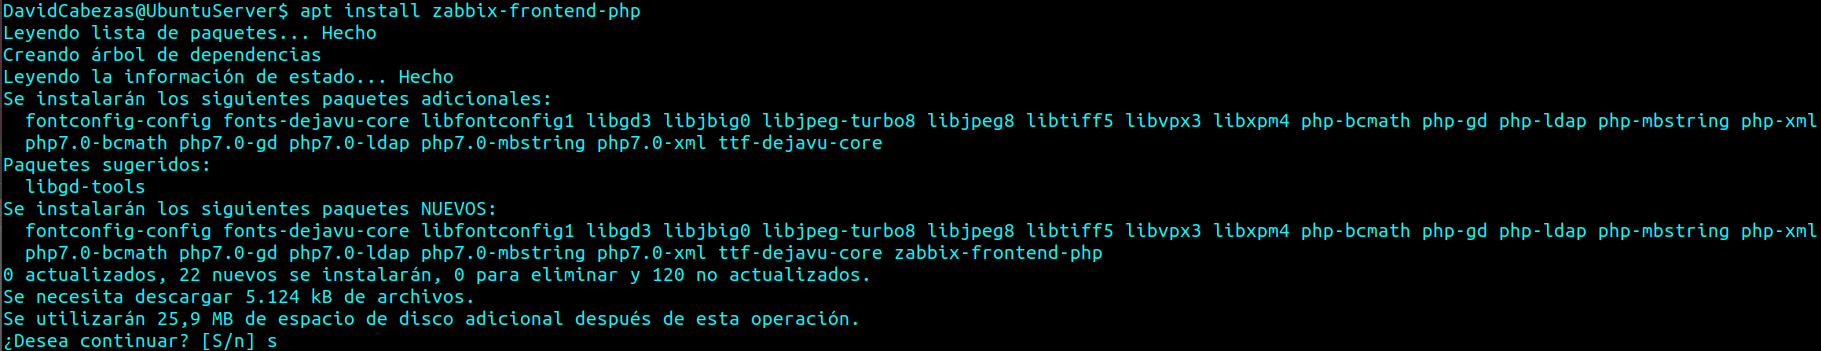
\includegraphics[width=160mm]{screenshots/frontend_installation}
\end{figure}

Al final de la instalación nos avisa de que debemos recargar el
servicio de Apache2.

\begin{figure}[H]
  \centering
  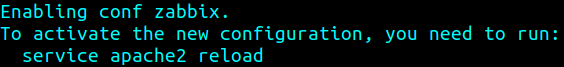
\includegraphics[width=100mm]{screenshots/aviso_apache2_reload}
\end{figure}

\begin{figure}[H]
  \centering
  
\includegraphics[width=100mm]{screenshots/apache2_reload}
\end{figure}

\subsubsection*{Crear base de datos}

Usaremos MySQL.

En este enlace se encuentran los comandos para hacerlo: \url{https://www.zabbix.com/documentation/3.4/manual/appendix/install/db_scripts#mysql}. Para entrar a MySQL como root, dejamos la contraseña en blanco.

\begin{figure}[H]
  \centering
  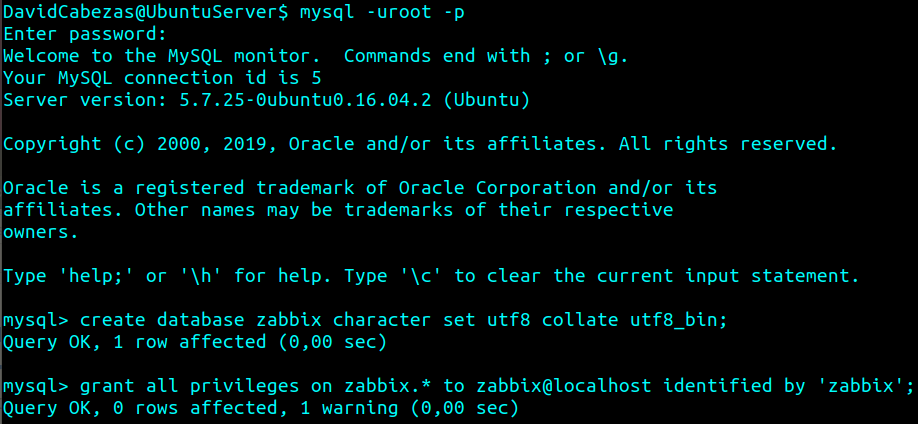
\includegraphics[width=160mm]{screenshots/server_create-database}
\end{figure}


\subsubsection*{Importamos datos}

Una vez creada la base de datos, continuamos siguiendo las
instrucciones de la guía anterior. Entramos a MySQL con el usuario y la contraseña que acabamos de crear (zabbix, zabbix).

\begin{figure}[H]
  \centering
  
\includegraphics[width=160mm]{screenshots/server_importing-data}
\end{figure}

\newpage

\subsubsection*{Configuración de la base de datos}

Modificamos el archivo de configuración y ponemos el host, usuario,
nombre de la BD y contraseña correspondientes:

\begin{figure}[H]
  \centering
  
\includegraphics[width=140mm]{screenshots/vi_server_database-conf}
\end{figure}

\begin{figure}[H]
  \centering
  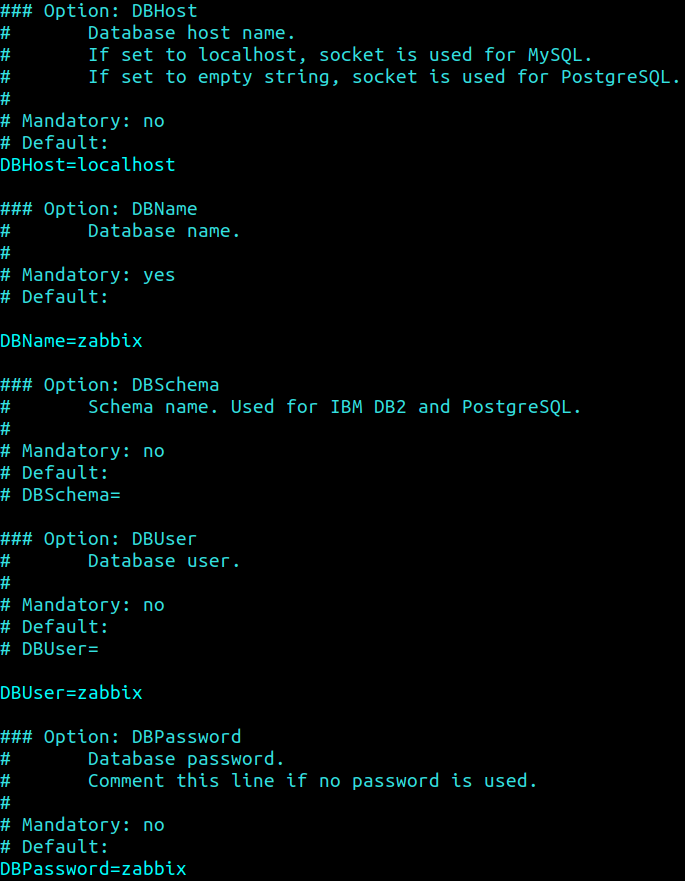
\includegraphics[width=140mm]{screenshots/server_config-database}
\end{figure}


\subsubsection*{Lanzar servicio y configurarlo para que se active en
  el arranque}

\begin{figure}[H]
  \centering
  
\includegraphics[width=140mm]{screenshots/start-boot}
\end{figure}

\subsubsection*{Configuración frontend}

Modificamos el archivo de configuración del frontend para poner la
zona horaria correcta

\begin{figure}[H]
  \centering
  
\includegraphics[width=160mm]{screenshots/vi_frontend-timezone}
\end{figure}

\begin{figure}[H]
  \centering
  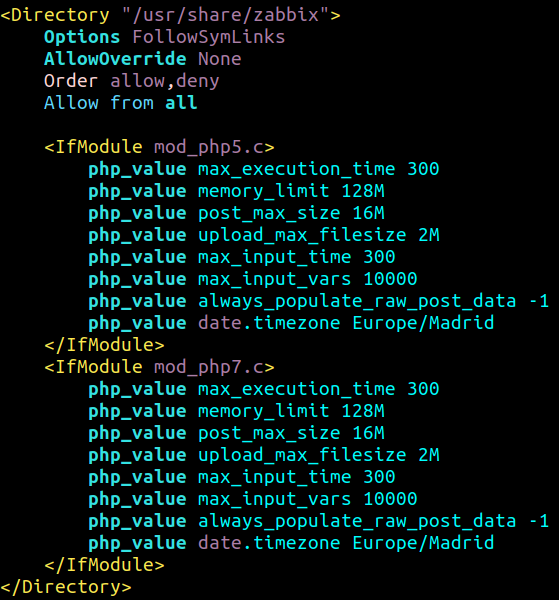
\includegraphics[width=120mm]{screenshots/frontend-timezone}
\end{figure}

\newpage

\subsubsection*{Instalación de frontend}

Ahora seguimos las instrucciones del enlace
\url{https://www.zabbix.com/documentation/3.4/manual/installation/install#installing_frontend}
para la correcta instalación del frontend. \\

Resumen de la instalación:

\begin{figure}[H]
  \centering
  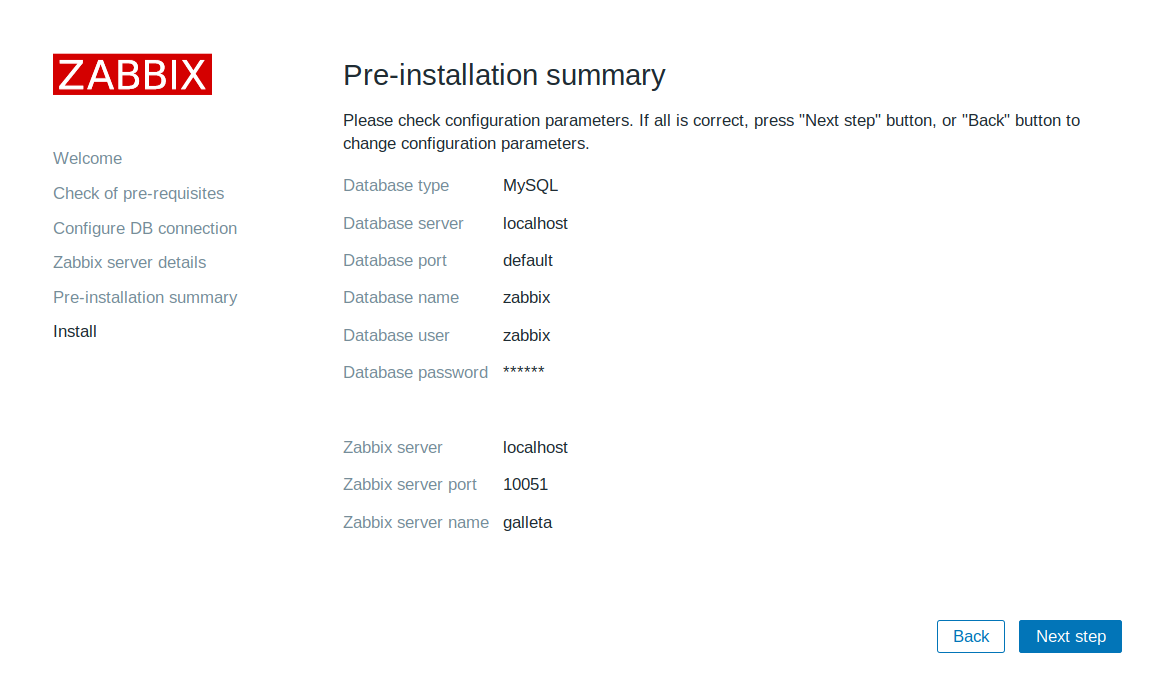
\includegraphics[width=140mm]{screenshots/frontend-summary}
\end{figure}

Seguidamente nos pide usuario y contraseña, que por defecto son Admin
y zabbix.

\begin{figure}[H]
  \centering
  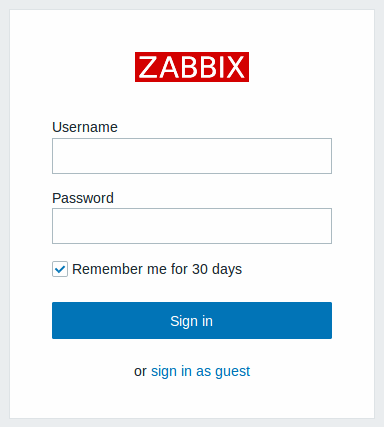
\includegraphics[width=100mm]{screenshots/login}
\end{figure}

Y ya estamos en la dashboard

\begin{figure}[H]
  \centering
  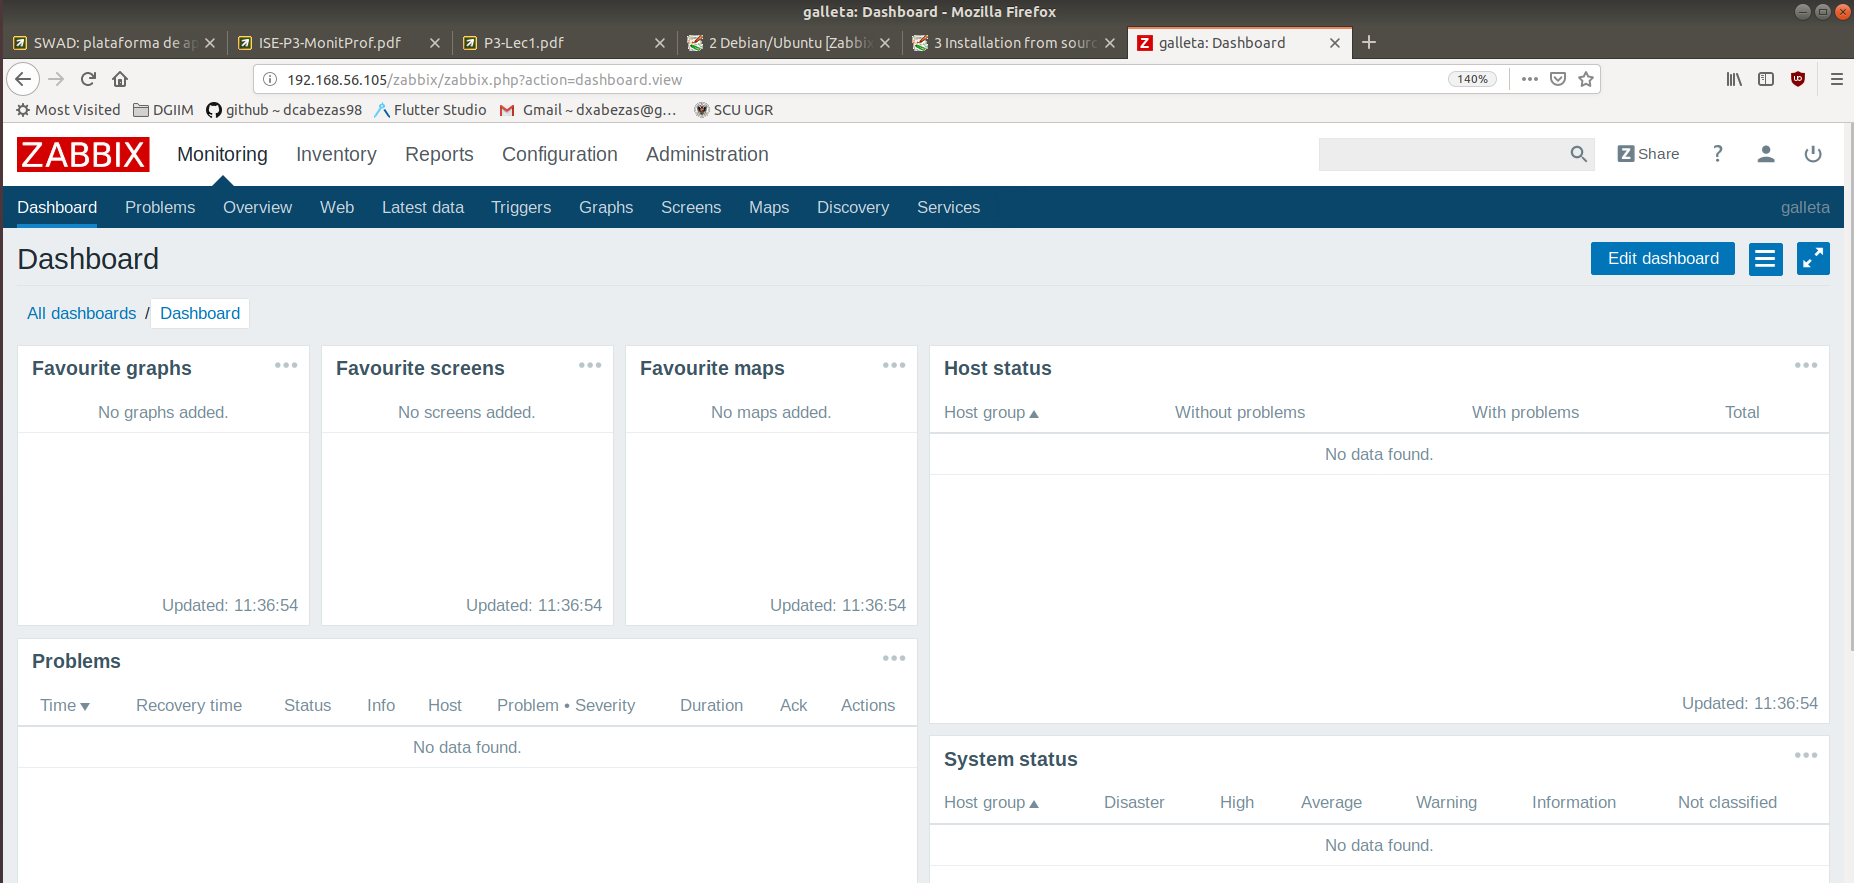
\includegraphics[width=140mm]{screenshots/dashboard}
\end{figure}


\subsubsection*{Instalación del agente}

Instalamos y lanzamos el agente.

\begin{figure}[H]
  \centering
  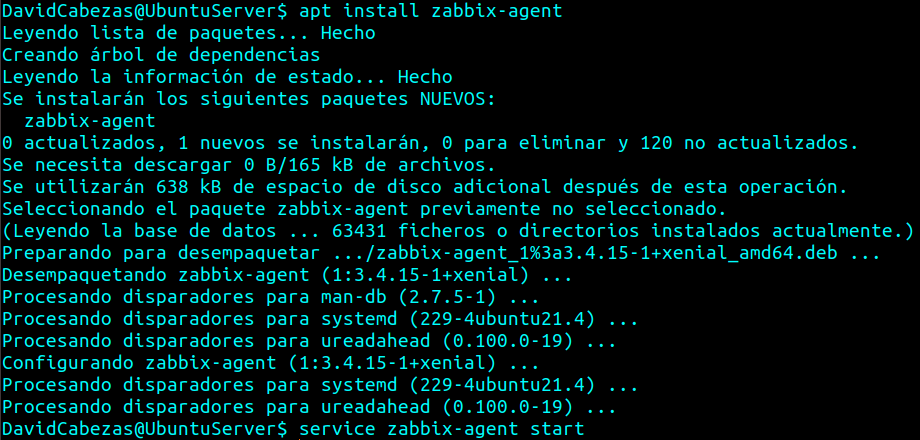
\includegraphics[width=140mm]{screenshots/agent_installation}
\end{figure}

Instalamos la utilidad zabbix\_get para probar comprobar que el agente
funciona.

\begin{figure}[H]
  \centering
  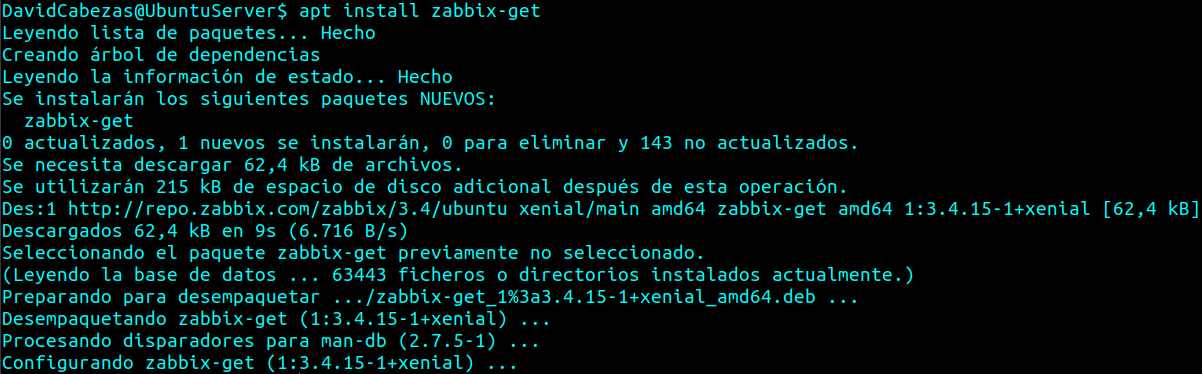
\includegraphics[width=160mm]{screenshots/zabbix-get}
\end{figure}

\begin{figure}[H]
  \centering
  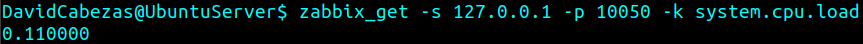
\includegraphics[width=140mm]{screenshots/zabbix_get}
\end{figure}

\subsubsection*{Configuración del agente}

\begin{figure}[H]
  \centering
  
\includegraphics[width=140mm]{screenshots/us_vi_agent-conf}
\end{figure}

\begin{figure}[H]
  \centering
  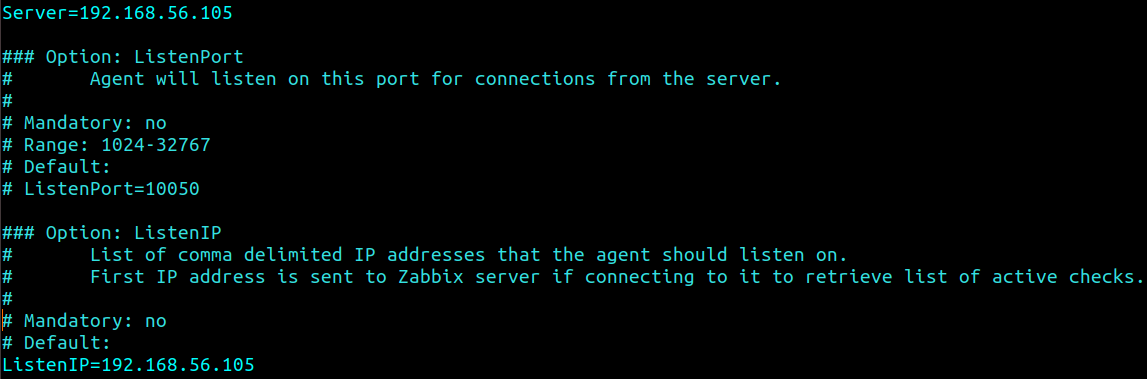
\includegraphics[width=160mm]{screenshots/us_agent-conf}
\end{figure}

Lo volvemos a lanzar con \texttt{service zabbix-agent restart}

\subsubsection*{Habilitamos los puertos para Zabbix}

\begin{figure}[H]
  \centering
  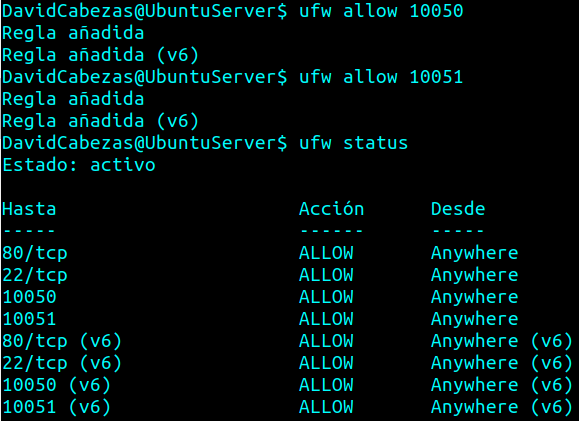
\includegraphics[width=120mm]{screenshots/ufw-allow}
\end{figure}

\newpage

\section{Instalación del agente en CentOS}

Siguiendo la documentación oficial
(\url{https://www.zabbix.com/documentation/3.4/manual/installation/install_from_packages/rhel_centos}),
descargo los paquetes e instalo el agente

\begin{figure}[H]
  \centering
  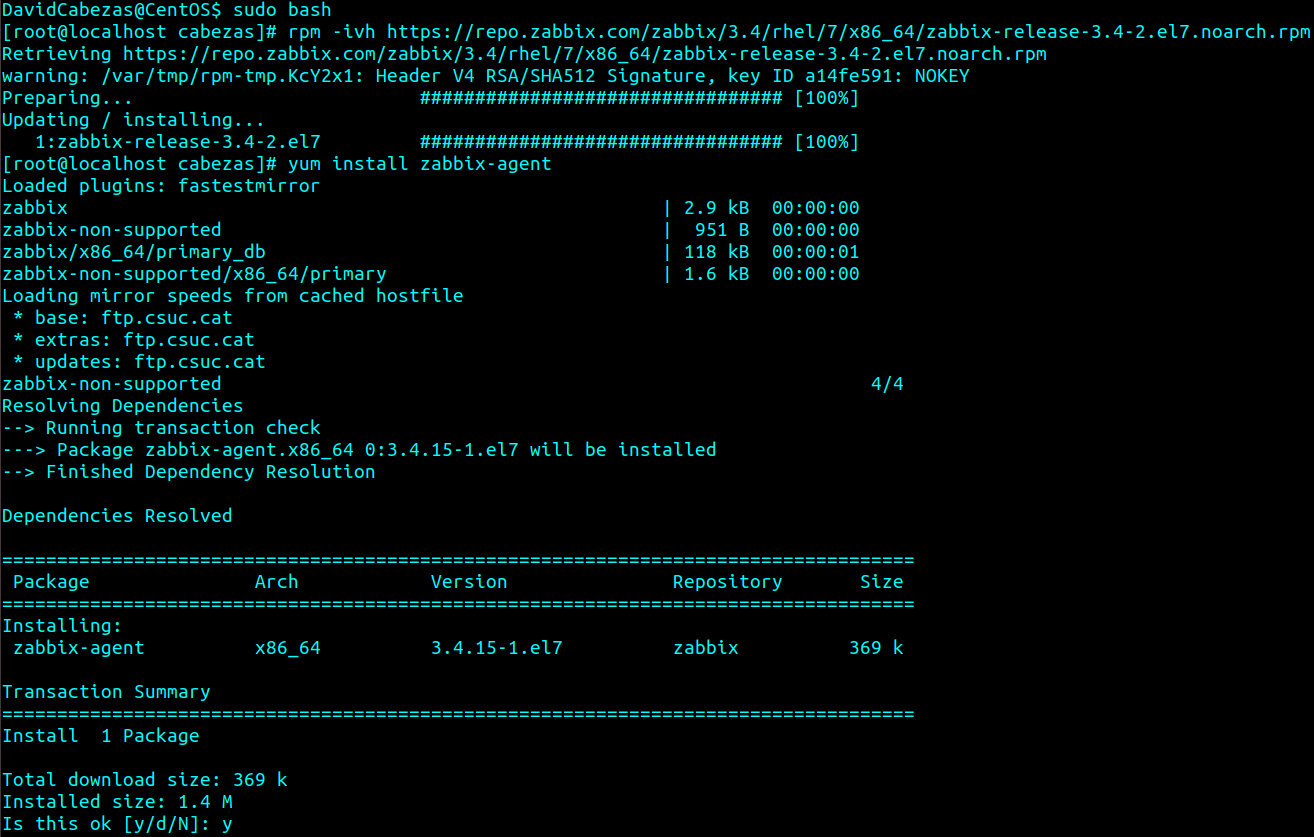
\includegraphics[width=170mm]{screenshots/centos_installation}
\end{figure}

Ahora voy a lanzar el agente, pero no funciona

\begin{figure}[H]
  \centering
  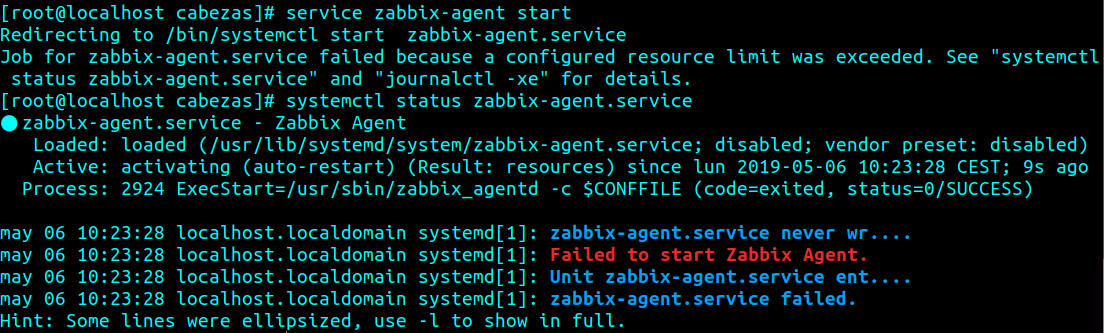
\includegraphics[width=160mm]{screenshots/centos_error-selinux}
\end{figure}

La documentación nos advierte de que si tenemos SELinux en enforcing,
el agente no arrancará a no ser que cambiemos la configuración. Así
que procederé a desabilitar SELinux como indica en este enlace: \url{https://support.zabbix.com/browse/ZBX-14922}

\begin{figure}[H]
  \centering
  
\includegraphics[width=120mm]{screenshots/vi_selinux}
\end{figure}

\begin{figure}[H]
  \centering
  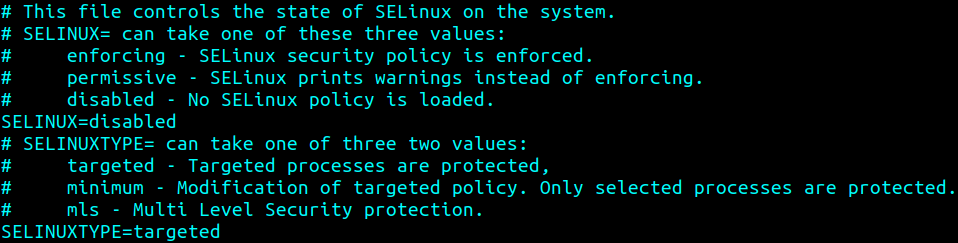
\includegraphics[width=160mm]{screenshots/selinux-config}
\end{figure}

Ya podemos lanzar el agente

\begin{figure}[H]
  \centering
  
\includegraphics[width=140mm]{screenshots/centos_start-agent}
\end{figure}

\subsubsection*{Modificamos el archivo de configuración del agente}

\begin{figure}[H]
  \centering
  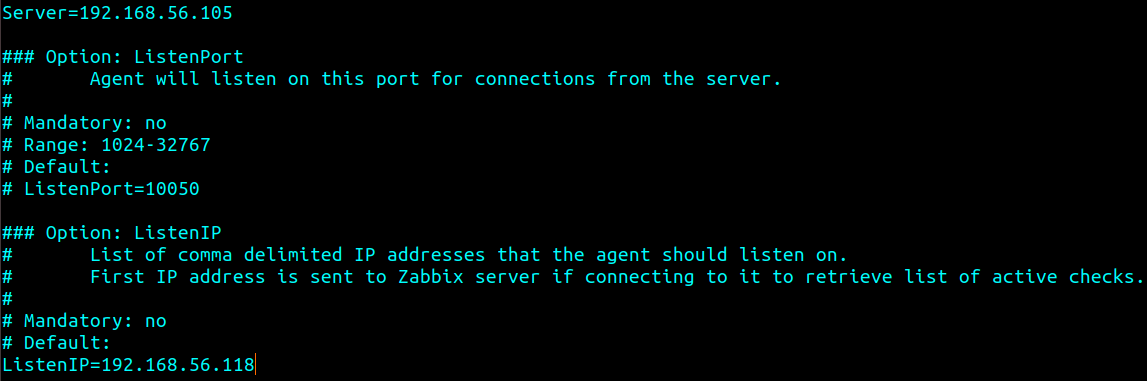
\includegraphics[width=160mm]{screenshots/centos_agent-conf}
\end{figure}


Ahora hay que volverlo a lanzar con \texttt{service zabbix-agent
  restart}. \\ Y finalmente habilitamos los puertos necesarios para el
funcionamiento del agente

\begin{figure}[H]
  \centering
  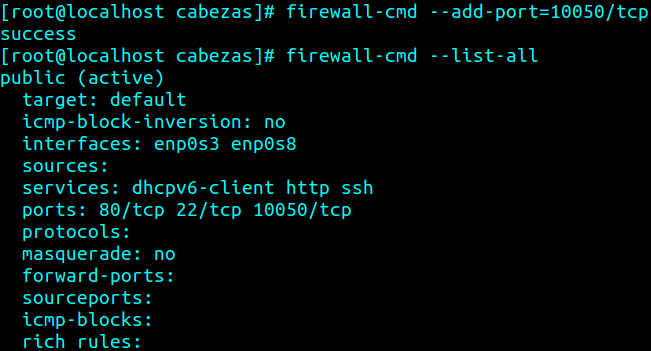
\includegraphics[width=140mm]{screenshots/firewall-cmd}
\end{figure}

\section{Monitorización}

\subsubsection*{Creamos hosts}

Seguimos las instrucciones de la documentación \url{https://www.zabbix.com/documentation/3.4/manual/quickstart/host}

\begin{figure}[H]
  \centering
  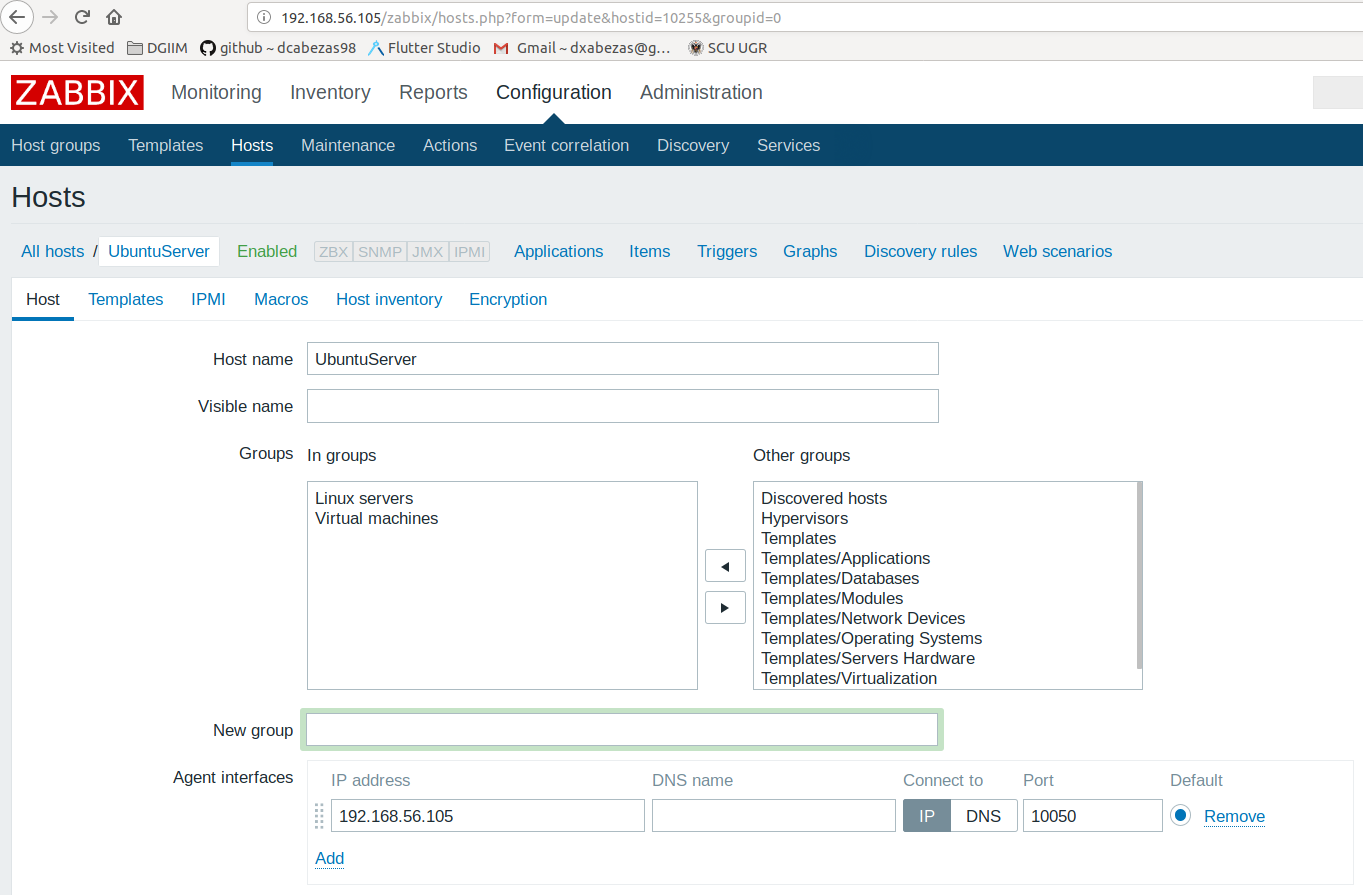
\includegraphics[width=140mm]{screenshots/new-host_us}
\end{figure}

\begin{figure}[H]
  \centering
  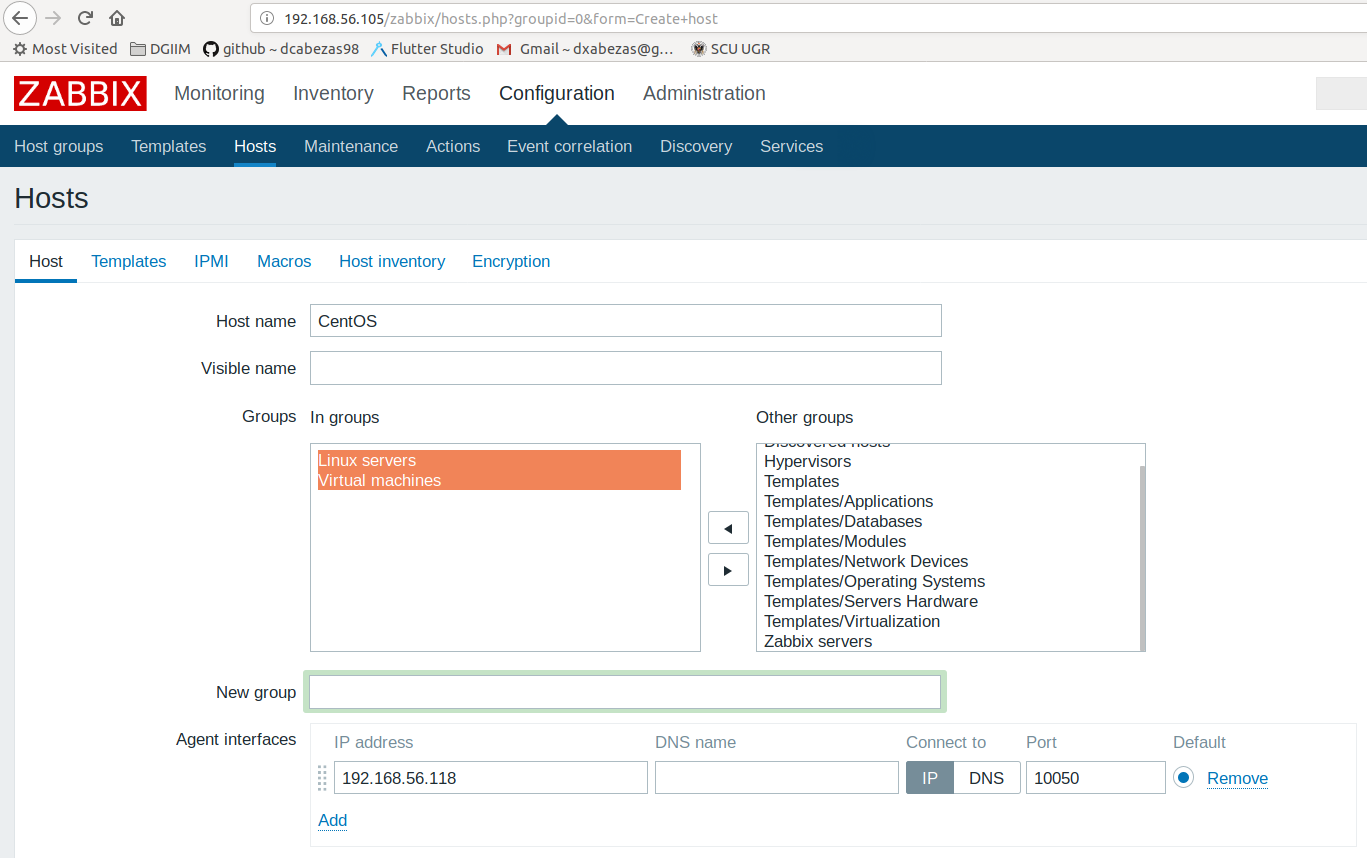
\includegraphics[width=140mm]{screenshots/new-host_centos}
\end{figure}

\newpage

\subsubsection*{Creamos items}

Seguimos el manual \url{https://www.zabbix.com/documentation/3.4/manual/quickstart/item}

Creamos los items para monitorizar SSH:

\begin{figure}[H]
  \centering
  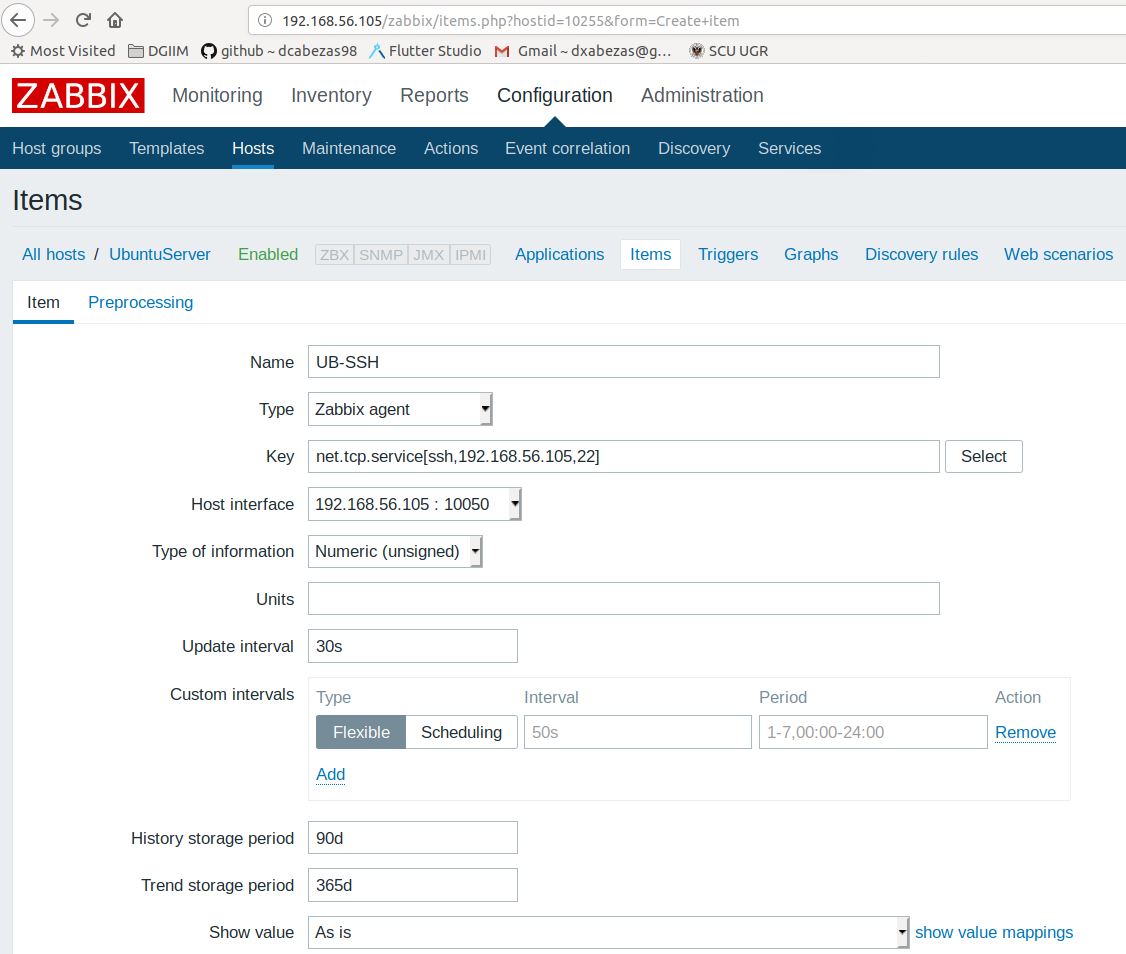
\includegraphics[width=120mm]{screenshots/item_us-ssh}
\end{figure}

\begin{figure}[H]
  \centering
  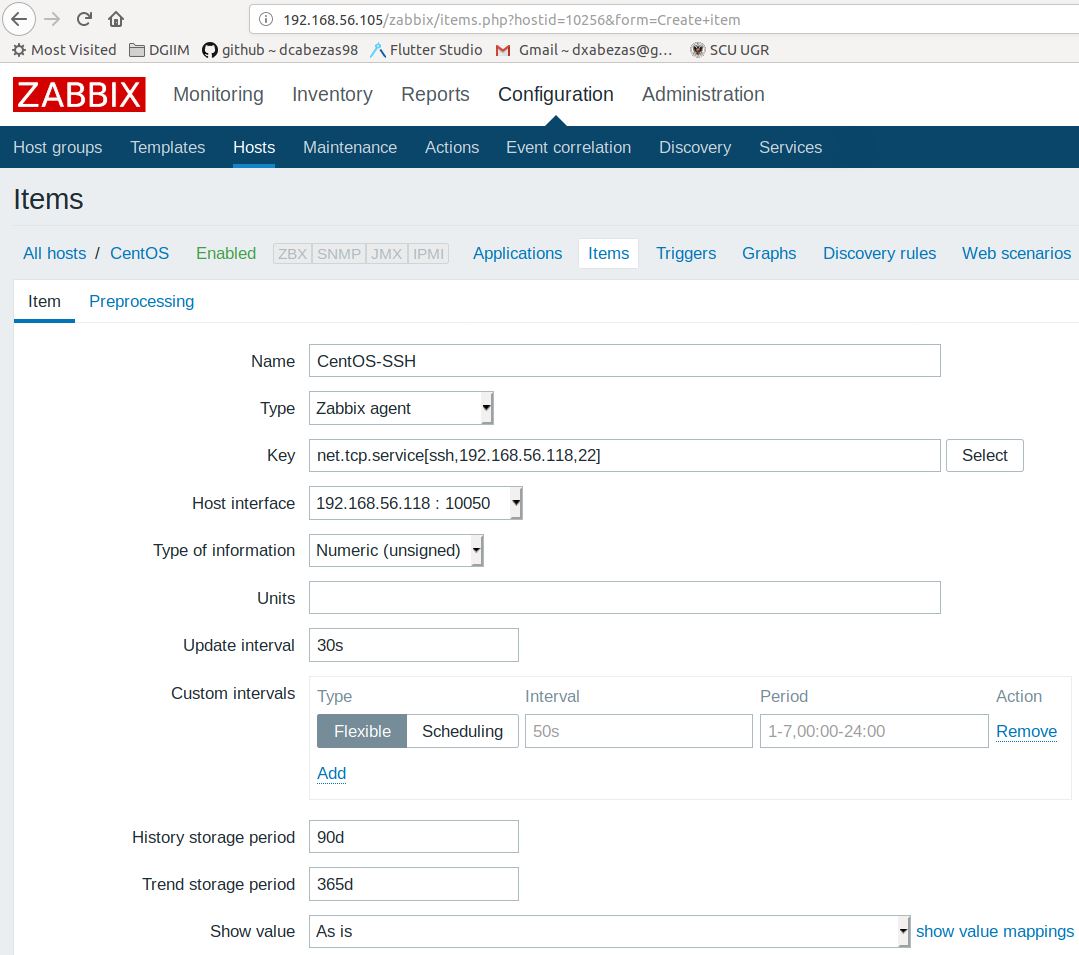
\includegraphics[width=120mm]{screenshots/item_centos-ssh}
\end{figure}

Para los items que monitorizan HTTP, he usado un template ya incluido:

\begin{figure}[H]
  \centering
  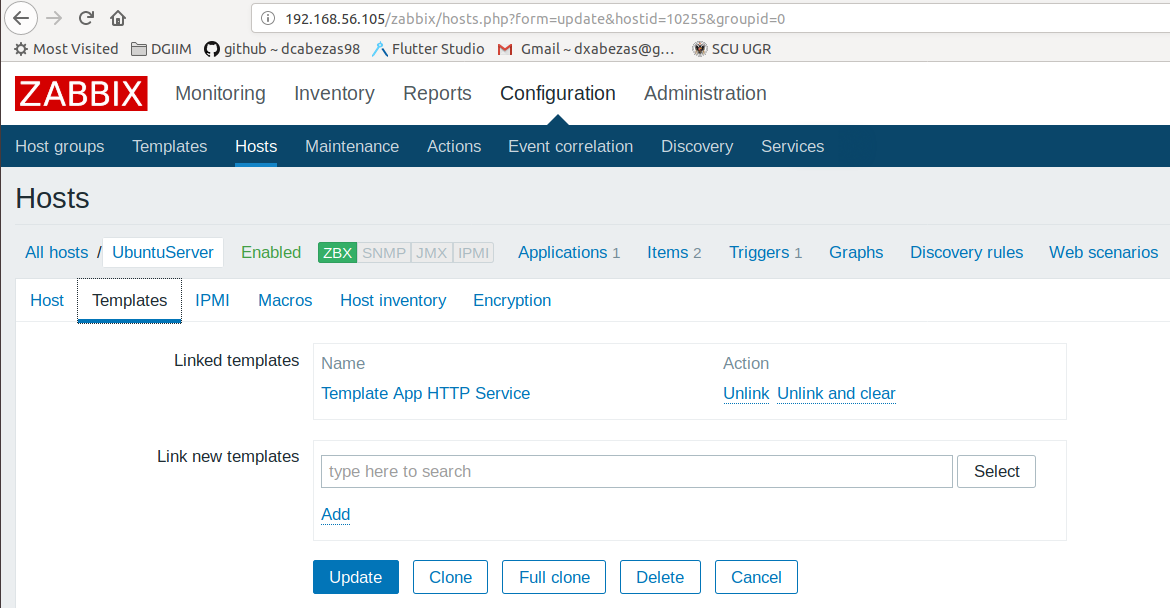
\includegraphics[width=120mm]{screenshots/item_us-http}
\end{figure}

\begin{figure}[H]
  \centering
  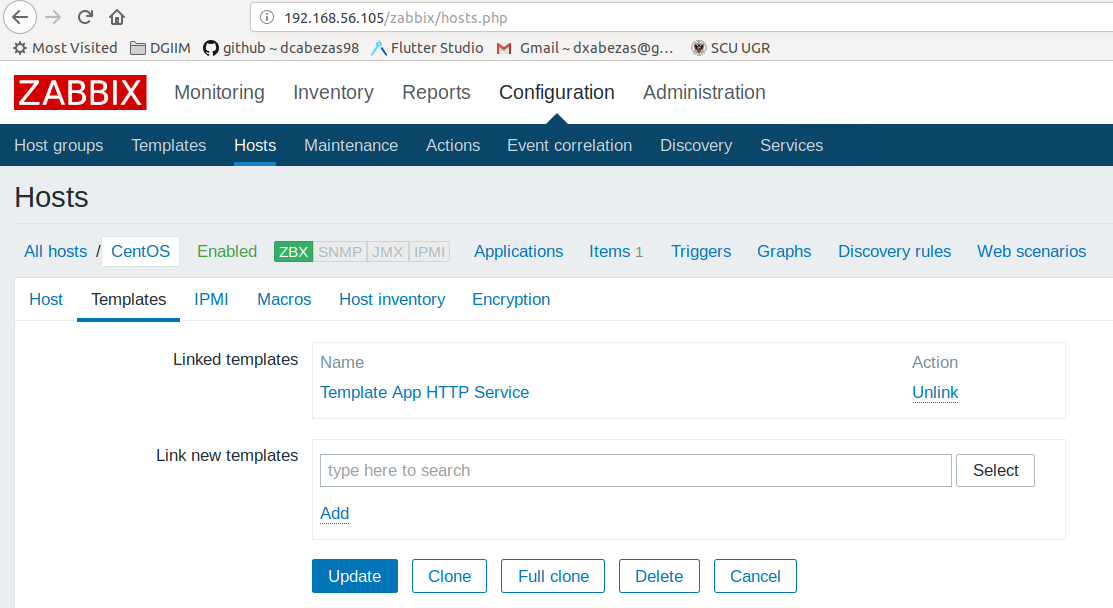
\includegraphics[width=120mm]{screenshots/item_centos-http}
\end{figure}

La ventana de hosts queda así

\begin{figure}[H]
  \centering
  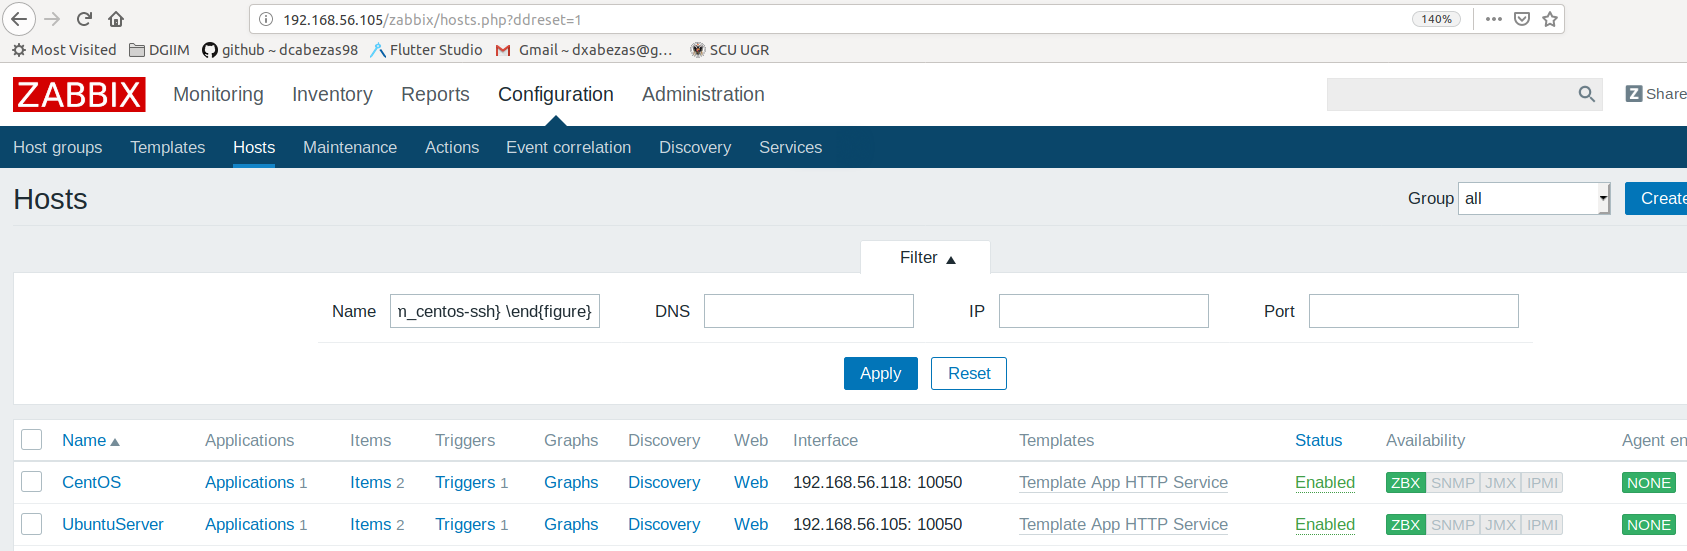
\includegraphics[width=160mm]{screenshots/hosts}
\end{figure}

Y ya podemos empezar a monitorizar, para ello vamos a Monitoring $\rightarrow$ Latest Data.

\begin{figure}[H]
  \centering
  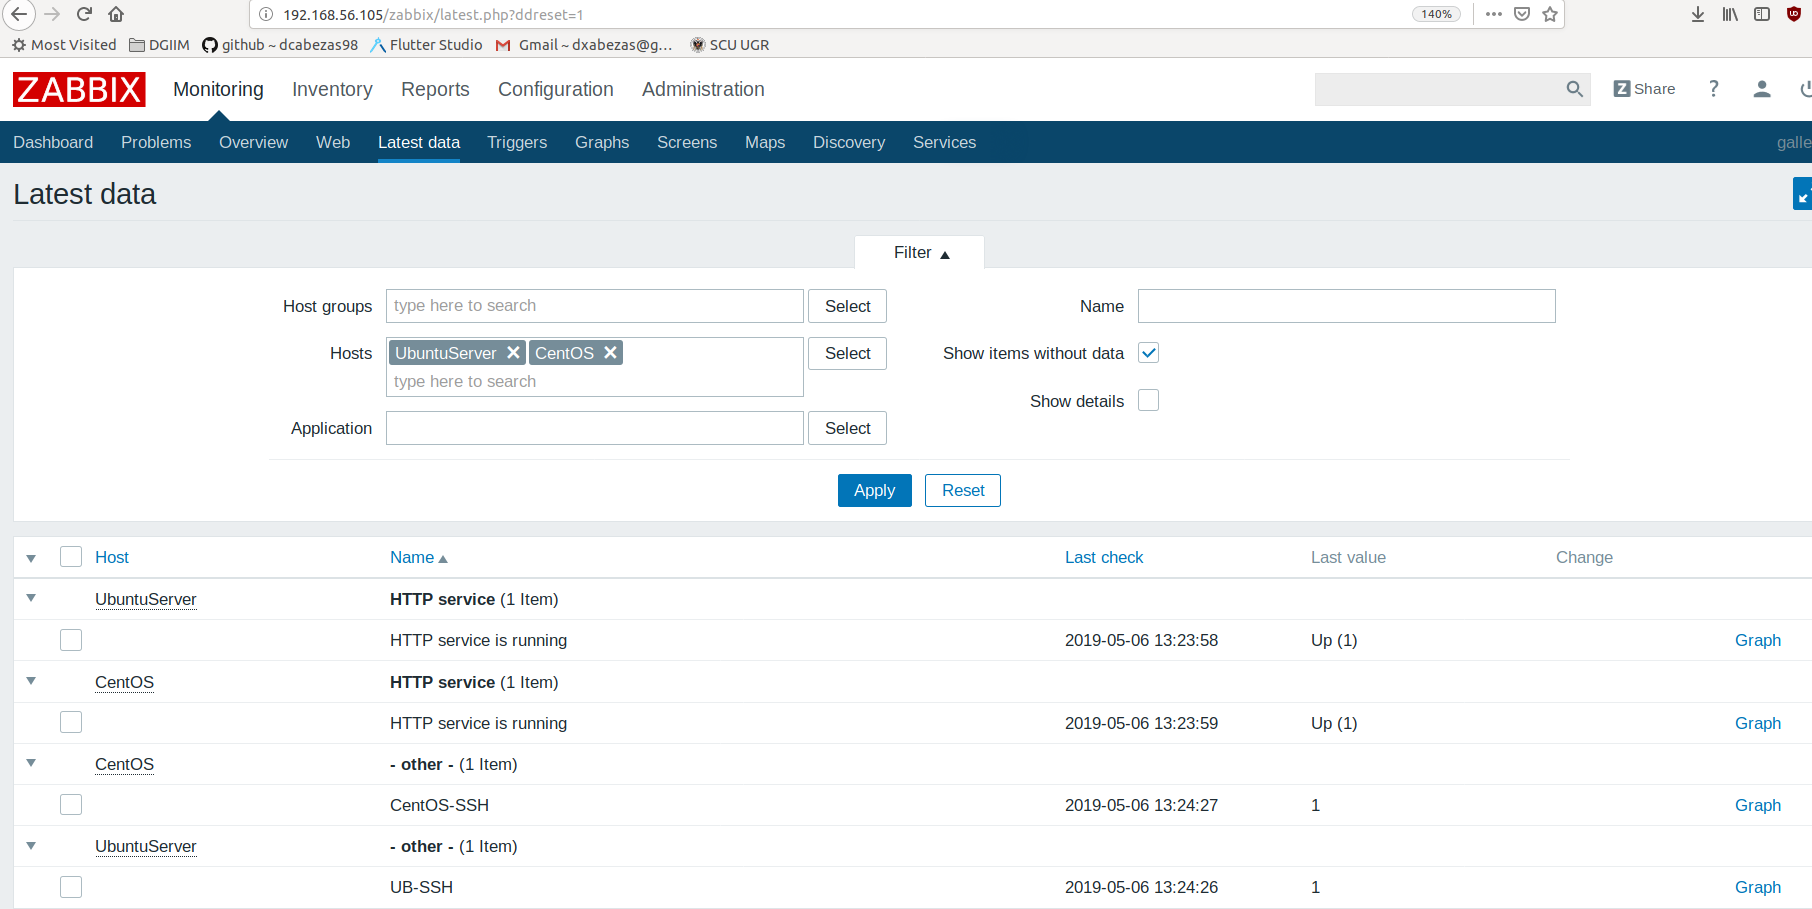
\includegraphics[width=160mm]{screenshots/latest-data}
\end{figure}

Haciendo clic en Graph, podemos visualizar los gráficos.

He ido usando \texttt{systemctl stop <servicio>} y \texttt{systemctl start <servicio>} para comprobar que monitorizaba correctamente.

\begin{figure}[H]
  \centering
  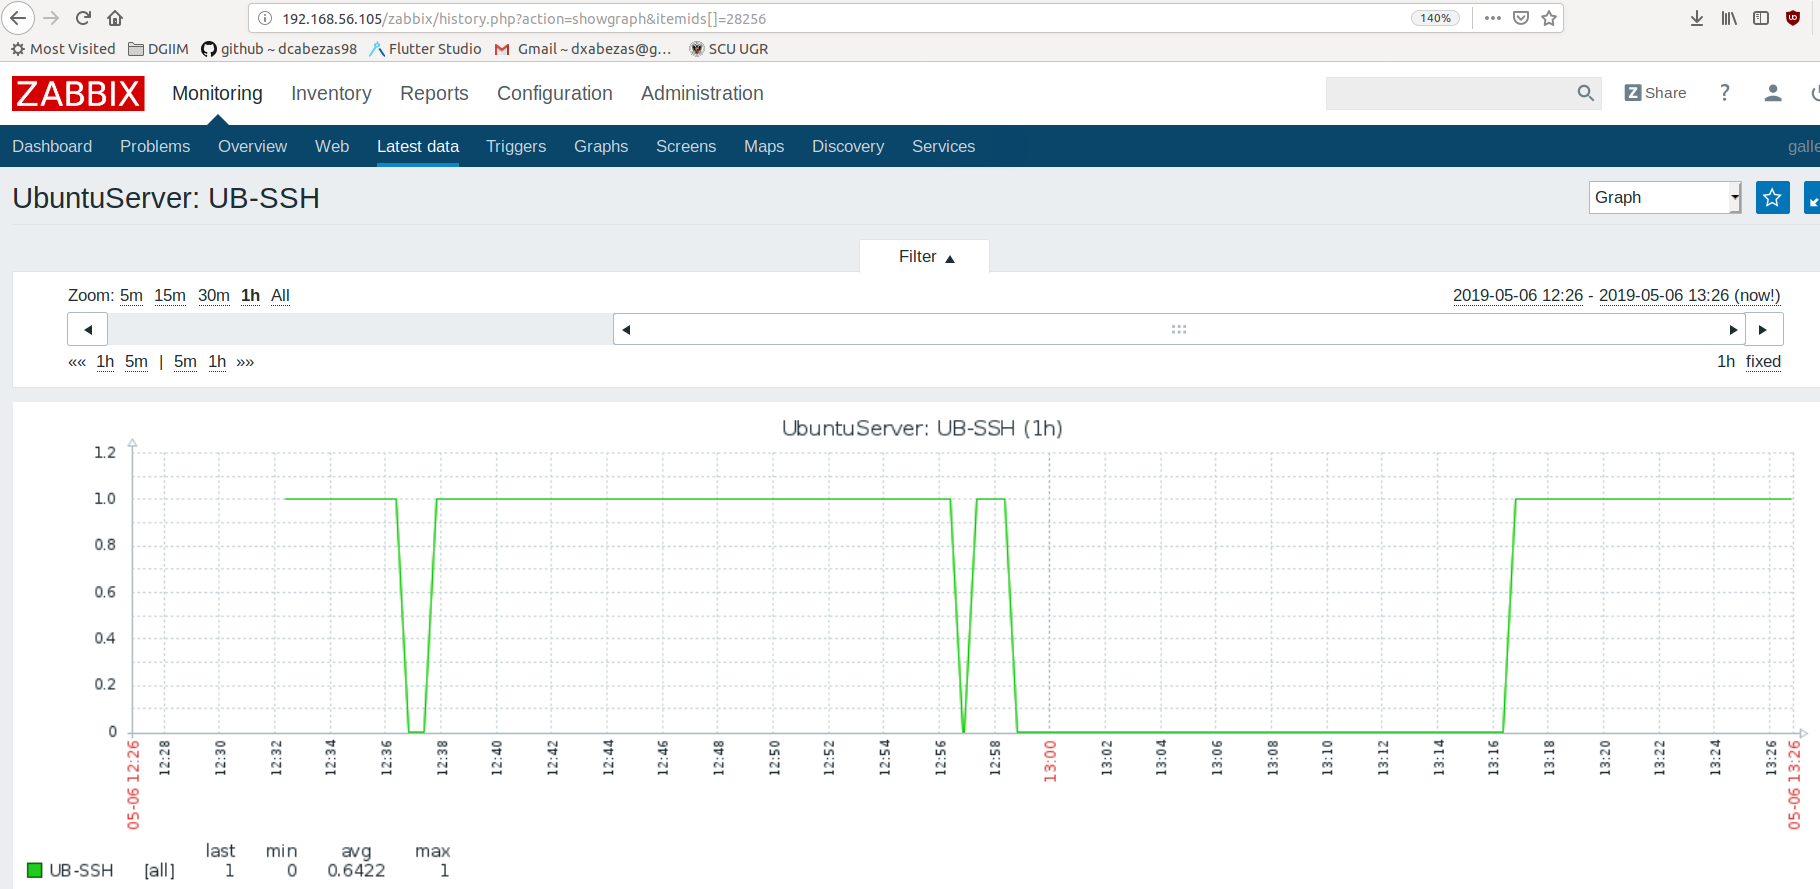
\includegraphics[width=150mm]{screenshots/graph_us-ssh}
\end{figure}

\begin{figure}[H]
  \centering
  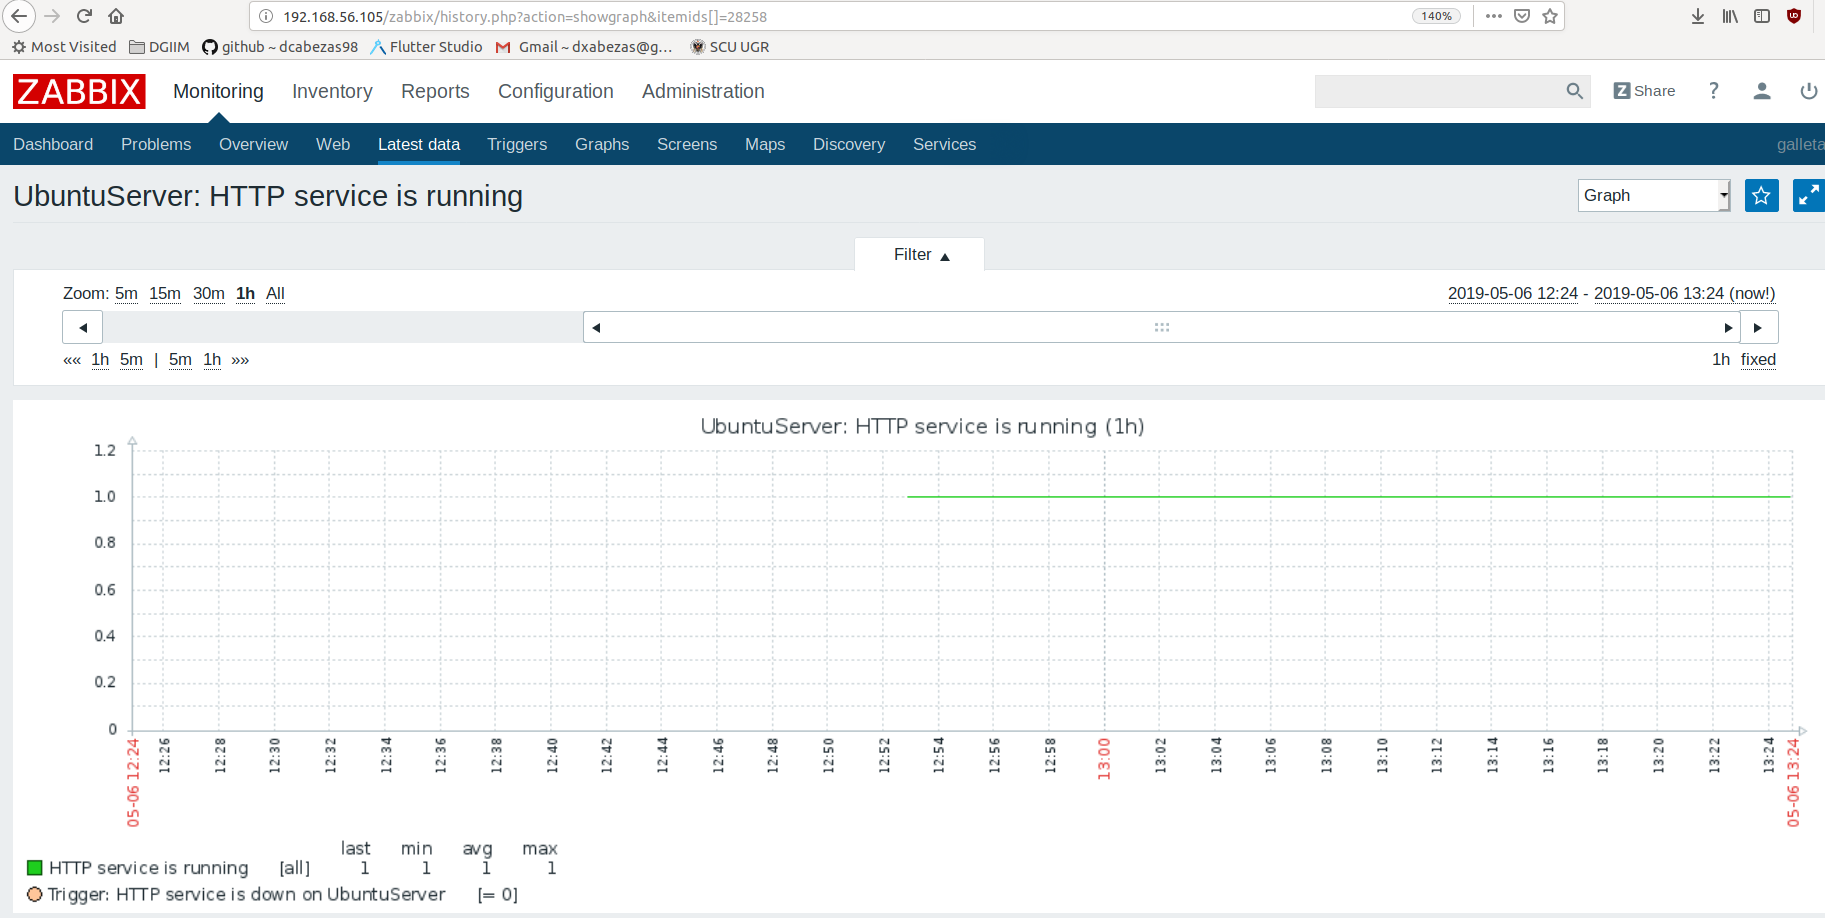
\includegraphics[width=150mm]{screenshots/graph_us-http}
\end{figure}

\begin{figure}[H]
  \centering
  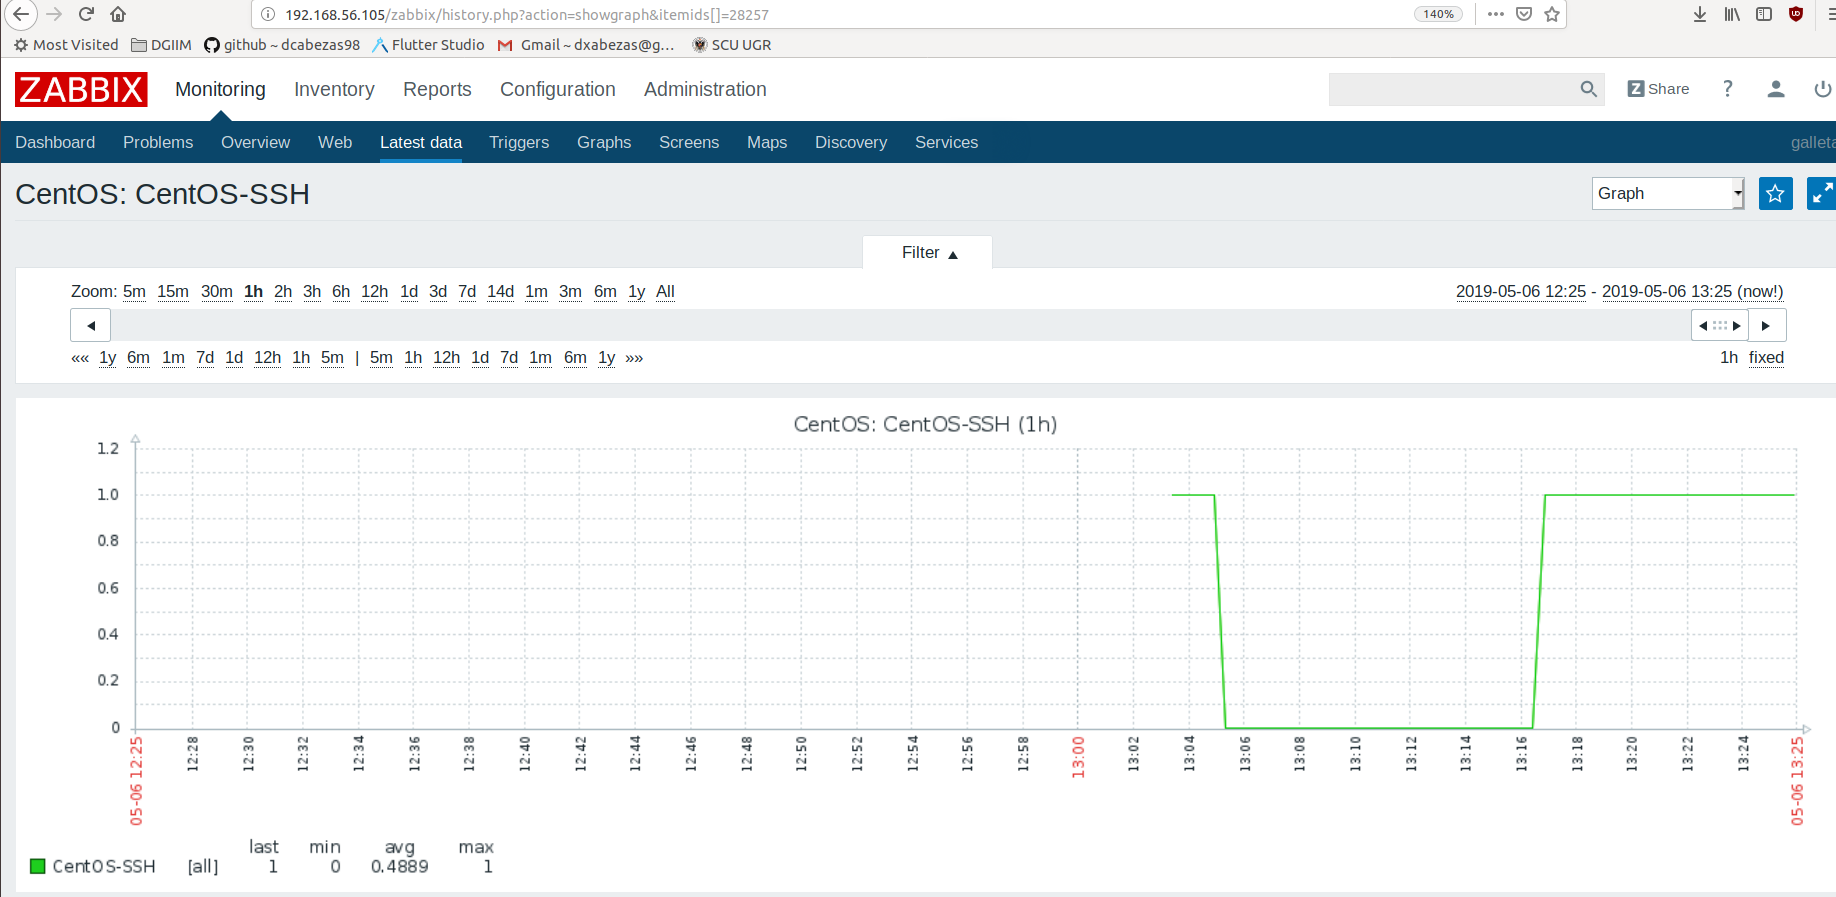
\includegraphics[width=150mm]{screenshots/graph_centos-ssh}
\end{figure}

\begin{figure}[H]
  \centering
  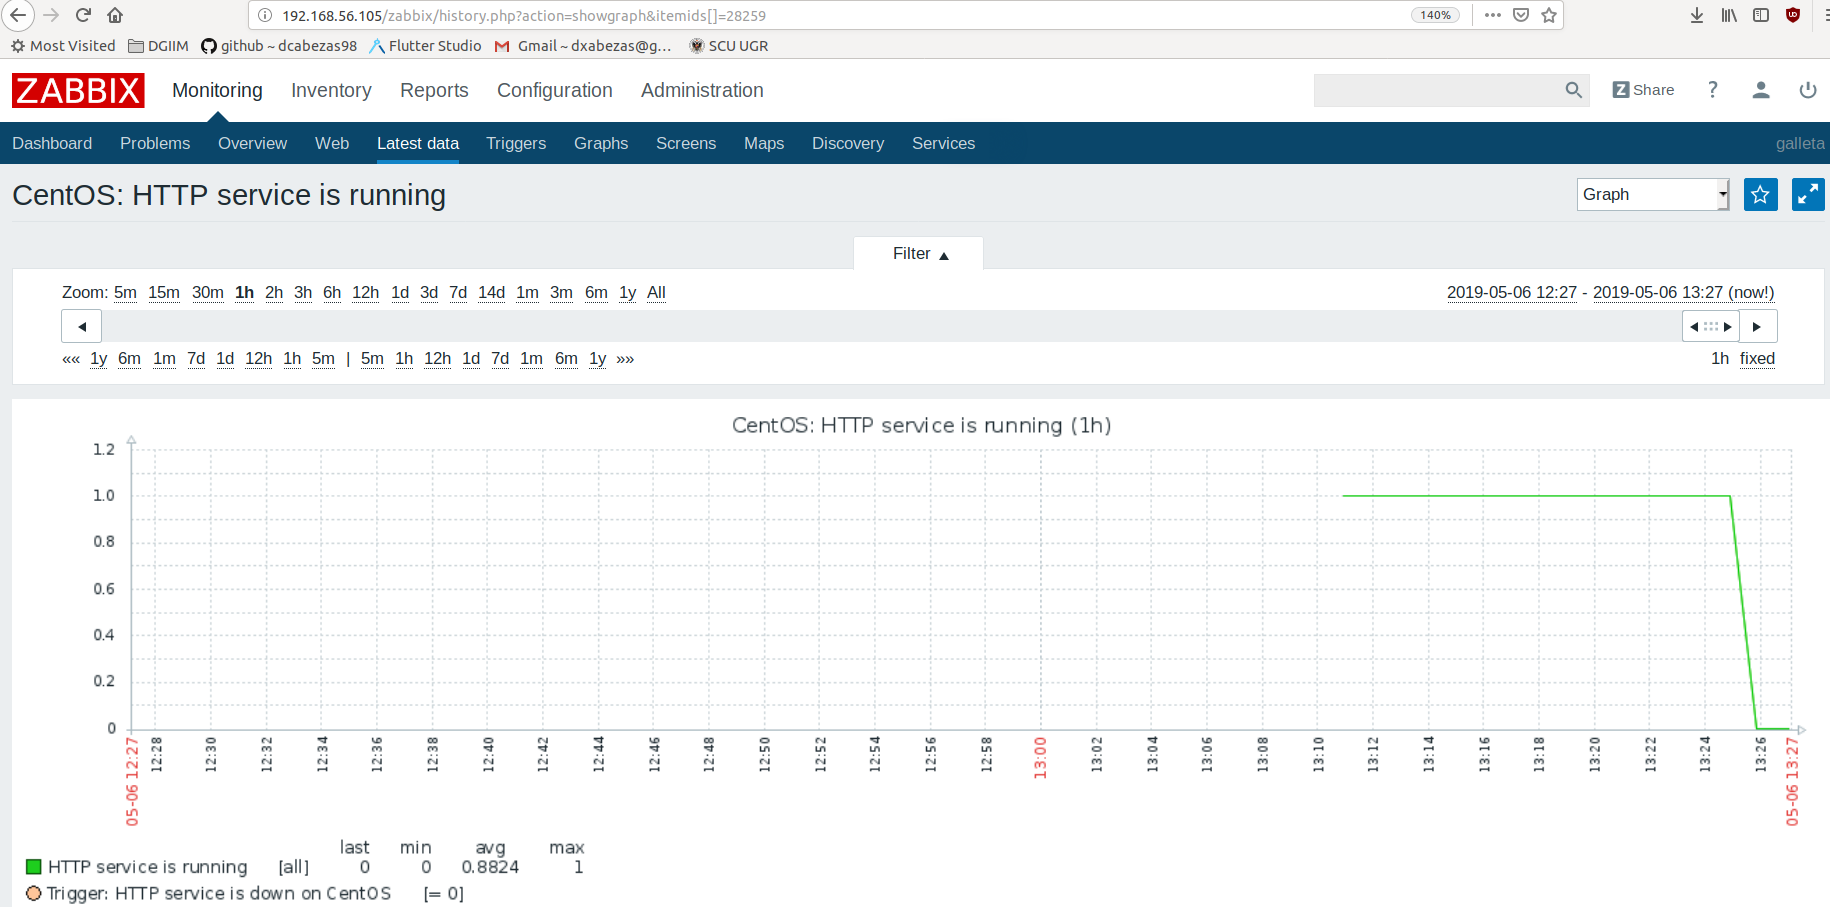
\includegraphics[width=150mm]{screenshots/graph_centos-http}
\end{figure}

\end{document}